%%**************************************************************
%% Vorlage fuer Praxisarbeiten (o.ä.) der DHBW
%%
%% Autor: Tobias Dreher, Yves Fischer
%% Datum: 06.07.2011
%%
%% Autor: Michael Gruben
%% Datum: 15.05.2013
%%
%% Autor: Markus Barthel
%% Datum: 22.08.2014
%%
%%Autor: Pascal Schröder
%%Datum: 27.03.2017
%%**************************************************************

%!TEX root = ../dokumentation.tex

%
% Nahezu alle Einstellungen koennen hier getaetigt werden
%

\RequirePackage[l2tabu, orthodox]{nag}	% weist in Commandozeile bzw. log auf veraltete LaTeX Syntax hin

\documentclass[%
	pdftex,
	oneside,			% Einseitiger Druck.
	12pt,				% Schriftgroesse
	parskip=half,		% Halbe Zeile Abstand zwischen Absätzen.
%	topmargin = 10pt,	% Abstand Seitenrand (Std:1in) zu Kopfzeile [laut log: unused]
	headheight = 14pt,	% Höhe der Kopfzeile
%	headsep = 30pt,	% Abstand zwischen Kopfzeile und Text Body  [laut log: unused]
	headsepline,		% Linie nach Kopfzeile.
	footsepline,		% Linie vor Fusszeile.
	footheight = 16pt,	% Höhe der Fusszeile
	abstracton,		% Abstract Überschriften
	DIV=calc,		% Satzspiegel berechnen
	BCOR=8mm,		% Bindekorrektur links: 8mm
	headinclude=false,	% Kopfzeile nicht in den Satzspiegel einbeziehen
	footinclude=false,	% Fußzeile nicht in den Satzspiegel einbeziehen
	listof=totoc,		% Abbildungs-/ Tabellenverzeichnis im Inhaltsverzeichnis darstellen
	toc=bibliography,	% Literaturverzeichnis im Inhaltsverzeichnis darstellen
]{scrreprt}	% Koma-Script report-Klasse, fuer laengere Bachelorarbeiten alternativ auch: scrbook

% Einstellungen laden
\usepackage{xstring}
\usepackage[utf8]{inputenc}
\usepackage[T1]{fontenc}

\newcommand{\einstellung}[1]{%
  \expandafter\newcommand\csname #1\endcsname{}
  \expandafter\newcommand\csname setze#1\endcsname[1]{\expandafter\renewcommand\csname#1\endcsname{##1}}
}
\newcommand{\langstr}[1]{\einstellung{lang#1}}

\einstellung{matrikelnr}
\einstellung{titel}
\einstellung{kurs}
\einstellung{datumAbgabe}
\einstellung{firma}
\einstellung{firmenort}
\einstellung{abgabeort}
\einstellung{studiengang}
\einstellung{dhbw}
\einstellung{abteilung}
\einstellung{betreuer}
\einstellung{spaceline}
\einstellung{zeitraum}
\einstellung{arbeit}
\einstellung{autor}
\einstellung{sprache}
\einstellung{schriftart}
\einstellung{seitenrand}
\einstellung{kapitelabstand}
\einstellung{spaltenabstand}
\einstellung{zeilenabstand}
\einstellung{zitierstil}
 % verfügbare Einstellungen
%%%%%%%%%%%%%%%%%%%%%%%%%%%%%%%%%%%%%%%%%%%%%%%%%%%%%%%%%%%%%%%%%%%%%%%%%%%%%%%
%                                   Einstellungen
%
% Hier können alle relevanten Einstellungen für diese Arbeit gesetzt werden.
% Dazu gehören Angaben u.a. über den Autor sowie Formatierungen.
%
%
%%%%%%%%%%%%%%%%%%%%%%%%%%%%%%%%%%%%%%%%%%%%%%%%%%%%%%%%%%%%%%%%%%%%%%%%%%%%%%%


%%%%%%%%%%%%%%%%%%%%%%%%%%%%%%%%%%%% Sprache %%%%%%%%%%%%%%%%%%%%%%%%%%%%%%%%%%%
%% Aktuell sind Deutsch und Englisch unterstützt.
%% Es werden nicht nur alle vom Dokument erzeugten Texte in
%% der entsprechenden Sprache angezeigt, sondern auch weitere
%% Aspekte angepasst, wie z.B. die Anführungszeichen und
%% Datumsformate.
\setzesprache{en} % oder en
%%%%%%%%%%%%%%%%%%%%%%%%%%%%%%%%%%%%%%%%%%%%%%%%%%%%%%%%%%%%%%%%%%%%%%%%%%%%%%%%

%%%%%%%%%%%%%%%%%%%%%%%%%%%%%%%%%%% Angaben  %%%%%%%%%%%%%%%%%%%%%%%%%%%%%%%%%%%
%% Die meisten der folgenden Daten werden auf dem
%% Deckblatt angezeigt, einige auch im weiteren Verlauf
%% des Dokuments.
\setzematrikelnr{5501463}
\setzekurs{TINF16AI-BC}
\setzetitel{Experimental Study on Scalable Post-Groomer of the Wildfire HTAP System on Cloud}
\setzedatumAbgabe{09/24/2018}
\setzefirma{IBM Deutschland GmbH}
\setzefirmenort{San Jose - Almaden}
\setzeabgabeort{Mannheim}
\setzestudiengang{Applied Computer Science}
\setzedhbw{Mannheim}
\setzebetreuer{Yuanyuan Tian}
\setzeabteilung{IBM Research}
\setzezeitraum{05/07/2018 - 08/24/2018}
\setzearbeit{Project Report}
\setzeautor{Pascal Schroeder}
\setzespaceline{}
%%%%%%%%%%%%%%%%%%%%%%%%%%%%%%%%%%%%%%%%%%%%%%%%%%%%%%%%%%%%%%%%%%%%%%%%%%%%%%%%

%%%%%%%%%%%%%%%%%%%%%%%%%%%% Literaturverzeichnis %%%%%%%%%%%%%%%%%%%%%%%%%%%%%%
%% Bei Fehlern während der Verarbeitung bitte in ads/header.tex bei der
%% Einbindung des Pakets biblatex (ungefähr ab Zeile 110,
%% einmal für jede Sprache), biber in bibtex ändern.
\newcommand{\ladeliteratur}{%
\addbibresource{bibliographie.bib}
%\addbibresource{weitereDatei.bib}
}
%% Zitierstil
%% siehe: http://ctan.mirrorcatalogs.com/macros/latex/contrib/biblatex/doc/biblatex.pdf (3.3.1 Citation Styles)
%% mögliche Werte z.B numeric-comp, alphabetic, authoryear
\setzezitierstil{numeric-comp}
%%%%%%%%%%%%%%%%%%%%%%%%%%%%%%%%%%%%%%%%%%%%%%%%%%%%%%%%%%%%%%%%%%%%%%%%%%%%%%%%

%%%%%%%%%%%%%%%%%%%%%%%%%%%%%%%%% Layout %%%%%%%%%%%%%%%%%%%%%%%%%%%%%%%%%%%%%%%
%% Verschiedene Schriftarten
% laut nag Warnung: palatino obsolete, use mathpazo, helvet (option scaled=.95), courier instead
\setzeschriftart{lmodern} % palatino oder goudysans, lmodern, libertine

%% Paket um Textteile drehen zu können
\usepackage{rotating}
%% Paket um Seite im Querformat anzuzeigen
\usepackage{lscape}

%% Seitenränder
\setzeseitenrand{2.5cm}

%% Abstand vor Kapitelüberschriften zum oberen Seitenrand
\setzekapitelabstand{16pt}

%% Spaltenabstand
\setzespaltenabstand{10pt}
%%Zeilenabstand innerhalb einer Tabelle
\setzezeilenabstand{1.5}
%%%%%%%%%%%%%%%%%%%%%%%%%%%%%%%%%%%%%%%%%%%%%%%%%%%%%%%%%%%%%%%%%%%%%%%%%%%%%%%%

%%%%%%%%%%%%%%%%%%%%%%%%%%%%% Verschiedenes  %%%%%%%%%%%%%%%%%%%%%%%%%%%%%%%%%%%
%% Farben (Angabe in HTML-Notation mit großen Buchstaben)
\newcommand{\ladefarben}{%
	\definecolor{LinkColor}{HTML}{00007A}
	\definecolor{ListingBackground}{HTML}{FCF7DE}
}
%% Mathematikpakete benutzen (Pakete aktivieren)
%\usepackage{amsmath}
%\usepackage{amssymb}

%% Programmiersprachen Highlighting (Listings)
\newcommand{\listingsettings}{%
	\lstset{%
		language=Java,			% Standardsprache des Quellcodes
		numbers=left,			% Zeilennummern links
		stepnumber=1,			% Jede Zeile nummerieren.
		numbersep=5pt,			% 5pt Abstand zum Quellcode
		numberstyle=\tiny,		% Zeichengrösse 'tiny' für die Nummern.
		breaklines=true,		% Zeilen umbrechen wenn notwendig.
		breakautoindent=true,	% Nach dem Zeilenumbruch Zeile einrücken.
		postbreak=\space,		% Bei Leerzeichen umbrechen.
		tabsize=2,				% Tabulatorgrösse 2
		basicstyle=\ttfamily\footnotesize, % Nichtproportionale Schrift, klein für den Quellcode
		showspaces=false,		% Leerzeichen nicht anzeigen.
		showstringspaces=false,	% Leerzeichen auch in Strings ('') nicht anzeigen.
		extendedchars=true,		% Alle Zeichen vom Latin1 Zeichensatz anzeigen.
		captionpos=b,			% sets the caption-position to bottom
		backgroundcolor=\color{ListingBackground}, % Hintergrundfarbe des Quellcodes setzen.
		xleftmargin=0pt,		% Rand links
		xrightmargin=0pt,		% Rand rechts
		frame=single,			% Rahmen an
		frameround=ffff,
		rulecolor=\color{darkgray},	% Rahmenfarbe
		fillcolor=\color{ListingBackground},
		keywordstyle=\color[rgb]{0.133,0.133,0.6},
		commentstyle=\color[rgb]{0.133,0.545,0.133},
		stringstyle=\color[rgb]{0.627,0.126,0.941}
	}
}
%%%%%%%%%%%%%%%%%%%%%%%%%%%%%%%%%%%%%%%%%%%%%%%%%%%%%%%%%%%%%%%%%%%%%%%%%%%%%%%%

%%%%%%%%%%%%%%%%%%%%%%%%%%%%%%%% Eigenes %%%%%%%%%%%%%%%%%%%%%%%%%%%%%%%%%%%%%%%
%% Hier können Ergänzungen zur Präambel vorgenommen werden (eigene Pakete, Einstellungen)



 % lese Einstellungen

\newcommand{\iflang}[2]{%
  \IfStrEq{\sprache}{#1}{#2}{}
}

\langstr{abkverz}
\langstr{anhang}
\langstr{glossar}
\langstr{deckblattabschlusshinleitung}
\langstr{artikelstudiengang}
\langstr{studiengang}
\langstr{anderdh}
\langstr{von}
\langstr{dbbearbeitungszeit}
\langstr{dbmatriknr}
\langstr{dbkurs}
\langstr{dbfirma}
\langstr{dbbetreuer}
\langstr{dbabteilung}
\langstr{dbbsigning}
\langstr{dbspaceline}
\langstr{sperrvermerk}
\langstr{formalien}
\langstr{abstractEN}
\langstr{abstractDE}
\langstr{listingname}
\langstr{listlistingname}
\langstr{listingautorefname}
 % verfügbare Strings
\input{lang/\sprache} % Übersetzung einlesen

% Einstellung der Sprache des Paketes Babel und der Verzeichnisüberschriften
\iflang{de}{\usepackage[english, ngerman]{babel}}
\iflang{en}{\usepackage[ngerman, english]{babel}} 


%%%%%%% Package Includes %%%%%%%

\usepackage[margin=\seitenrand,foot=1cm]{geometry}	% Seitenränder und Abstände
\usepackage[activate]{microtype} %Zeilenumbruch und mehr
\usepackage[onehalfspacing]{setspace}
\usepackage{makeidx}
\usepackage{tabularx}
\usepackage[autostyle=true,german=quotes]{csquotes}
\usepackage{longtable}
\usepackage{enumitem}	% mehr Optionen bei Aufzählungen
\usepackage{graphicx}
\usepackage{pdfpages}   % zum Einbinden von PDFs
\usepackage{xcolor} 	% für HTML-Notation
\usepackage{float}
\usepackage{array}
\usepackage{calc}		% zum Rechnen (Bildtabelle in Deckblatt)
\usepackage[right]{eurosym}
\usepackage{wrapfig}
\usepackage{pgffor} % für automatische Kapiteldateieinbindung
\usepackage[perpage, hang, multiple, stable]{footmisc} % Fussnoten
\usepackage[printonlyused]{acronym} % falls gewünscht kann die Option footnote eingefügt werden, dann wird die Erklärung nicht inline sondern in einer Fußnote dargestellt
\usepackage{listings}
\usepackage{fancyhdr}

% Notizen. Einsatz mit \todo{Notiz} oder \todo[inline]{Notiz}. 
\usepackage[obeyFinal,backgroundcolor=yellow,linecolor=black]{todonotes}
% Alle Notizen ausblenden mit der Option "final" in \documentclass[...] oder durch das auskommentieren folgender Zeile
% \usepackage[disable]{todonotes}

% Kommentarumgebung. Einsatz mit \comment{}. Alle Kommentare ausblenden mit dem Auskommentieren der folgenden und dem aktivieren der nächsten Zeile.
\newcommand{\comment}[1]{\par {\bfseries \color{blue} #1 \par}} %Kommentar anzeigen
% \newcommand{\comment}[1]{} %Kommentar ausblenden


%%%%%% Configuration %%%%%

%% Anwenden der Einstellungen

\usepackage{\schriftart}
\ladefarben{}

% Titel, Autor und Datum
\title{\titel}
\author{\autor}
\date{\datum}

% PDF Einstellungen
\usepackage[%
	pdftitle={\titel},
	pdfauthor={\autor},
	pdfsubject={\arbeit},
	pdfcreator={pdflatex, LaTeX with KOMA-Script},
	pdfpagemode=UseOutlines, 		% Beim Oeffnen Inhaltsverzeichnis anzeigen
	pdfdisplaydoctitle=true, 		% Dokumenttitel statt Dateiname anzeigen.
	pdflang={\sprache}, 			% Sprache des Dokuments.
]{hyperref}

% (Farb-)einstellungen für die Links im PDF
\hypersetup{%
	colorlinks=true, 		% Aktivieren von farbigen Links im Dokument
	linkcolor=LinkColor, 	% Farbe festlegen
	citecolor=LinkColor,
	filecolor=LinkColor,
	menucolor=LinkColor,
	urlcolor=LinkColor,
	linktocpage=false, 		% Nicht der Text sondern die Seitenzahlen in Verzeichnissen klickbar
	bookmarksnumbered=true 	% Überschriftsnummerierung im PDF Inhalt anzeigen.
}
% Workaround um Fehler in Hyperref, muss hier stehen bleiben
\usepackage{bookmark} %nur ein latex-Durchlauf für die Aktualisierung von Verzeichnissen nötig

% Schriftart in Captions etwas kleiner
\addtokomafont{caption}{\small}

% Literaturverweise (sowohl deutsch als auch englisch)
\iflang{de}{%
\usepackage[
	backend=biber,		% empfohlen. Falls biber Probleme macht: bibtex
	bibwarn=true,
	bibencoding=utf8,	% wenn .bib in utf8, sonst ascii
	sortlocale=de_DE,
	style=\zitierstil,
]{biblatex}
}
\iflang{en}{%
\usepackage[
	backend=biber,		% empfohlen. Falls biber Probleme macht: bibtex
	bibwarn=true,
	bibencoding=utf8,	% wenn .bib in utf8, sonst ascii
	sortlocale=en_US,
	style=\zitierstil,
]{biblatex}
}

\ladeliteratur{}

% Glossar
\usepackage[nonumberlist,toc]{glossaries}

%%%%%% Additional settings %%%%%%

% Hurenkinder und Schusterjungen verhindern
% http://projekte.dante.de/DanteFAQ/Silbentrennung
\clubpenalty = 10000 % schließt Schusterjungen aus (Seitenumbruch nach der ersten Zeile eines neuen Absatzes)
\widowpenalty = 10000 % schließt Hurenkinder aus (die letzte Zeile eines Absatzes steht auf einer neuen Seite)
\displaywidowpenalty=10000

% Bildpfad
\graphicspath{{images/}}

% Einige häufig verwendete Sprachen
\lstloadlanguages{PHP,Python,Java,C,C++,bash}
\listingsettings{}
% Umbennung des Listings
\renewcommand\lstlistingname{\langlistingname}
\renewcommand\lstlistlistingname{\langlistlistingname}
\def\lstlistingautorefname{\langlistingautorefname}

% Abstände in Tabellen
\setlength{\tabcolsep}{\spaltenabstand}
\renewcommand{\arraystretch}{\zeilenabstand}


\begin{document}

	% Deckblatt
	\begin{spacing}{1}
		%!TEX root = ../dokumentation.tex

\begin{titlepage}
	\begin{longtable}{p{8.2cm} p{5.4cm}}
		{\raisebox{\ht\strutbox-\totalheight}{
\includegraphics[height=2.5cm]{images/logo.png}}} &
		{\raisebox{\ht\strutbox-\totalheight}{
\includegraphics[height=2.5cm]{images/dhbw.png}}}
	\end{longtable}
	\enlargethispage{20mm}
	\begin{center}
		\vspace*{12mm}	{\LARGE\textbf \titel }\\
		\vspace*{12mm}	{\large\textbf \arbeit}\\
		\vspace*{12mm}	
		\vspace*{3mm}		
		\vspace*{12mm}	\langartikelstudiengang{} \langstudiengang{} \studiengang\\
    		\vspace*{3mm}		\langanderdh{} \dhbw\\
		\vspace*{12mm}	\langvon\\
		\vspace*{3mm}		{\large\textbf \autor}\\
		\vspace*{12mm}	\datumAbgabe\\
	\end{center}
	\vfill
	\begin{spacing}{1.2}
	\begin{tabbing}
		mmmmmmmmmmmmmmmmmmmmmmmmmm             \= \kill
		\textbf{\langdbbearbeitungszeit}       \>  \zeitraum\\
		\textbf{\langdbmatriknr, \langdbkurs}  \>  \matrikelnr, \kurs\\
		\textbf{\langdbabteilung}	\> \abteilung\\
		\textbf{\langdbfirma}                  \>  \firma, \firmenort\\
		\textbf{\langdbbetreuer}               \>  \betreuer\\
		\textbf{\langdbspaceline}		\>  \spaceline\\
		\textbf{\langdbbsigning}              \>	\rule{6cm}{0.4pt}
	\end{tabbing}
	\end{spacing}
\end{titlepage}

	\end{spacing}

	\pagestyle{fancyplain}
	\fancyhf{}
	\fancyhead[L]{
\includegraphics[height=0.8cm]{images/logo.png}}
	\fancyhead[R]{
\includegraphics[height=1cm]{images/dhbw.png}}
	\renewcommand{\headrulewidth}{0pt}
	
		% Sperrvermerk
		%%!TEX root = ../dokumentation.tex

\thispagestyle{empty}
% Sperrvermerk direkt hinter Titelseite
\section*{\langsperrvermerk}

\vspace*{2em}

\iflang{de}{%
  Die vorliegende {\arbeit} mit dem Titel {\itshape{} \titel{}\/} enthält unternehmensinterne bzw. vertrauliche Informationen der {\firma}, ist deshalb mit einem Sperrvermerk versehen und wird ausschließlich zu Prüfungszwecken am Studiengang {\studiengang} der Dualen Hochschule Baden-Württemberg {\dhbw} vorgelegt. Sie ist ausschließlich zur Einsicht durch den zugeteilten Gutachter, die Leitung des Studiengangs und ggf. den Prüfungsausschuss des Studiengangs bestimmt.  Es ist untersagt,
  \begin{itemize}
  \item den Inhalt dieser Arbeit (einschließlich Daten, Abbildungen, Tabellen, Zeichnungen usw.) als Ganzes oder auszugsweise weiterzugeben,
  \item Kopien oder Abschriften dieser Arbeit (einschließlich Daten, Abbildungen, Tabellen, Zeichnungen usw.) als Ganzes oder in Auszügen anzufertigen,
  \item diese Arbeit zu veröffentlichen bzw. digital, elektronisch oder virtuell zur Verfügung zu stellen. 
  \end{itemize}
Jede anderweitige Einsichtnahme und Veröffentlichung – auch von Teilen der Arbeit – bedarf der vorherigen Zustimmung durch den Verfasser und {\firma}.
}

%http://www.ib.dhbw-mannheim.de/fileadmin/ms/bwl-ib/Downloads_alt/Leitfaden_31.05.pdf

\iflang{en}{%
  The {\arbeit} on hand 
  \begin{center}{\itshape{} \titel{}\/}\end{center} 
   contains internal resp.\ confidential data of {\firma}. It is intended solely for inspection by the assigned examiner, the head of the {\studiengang} department and, if necessary, the Audit Committee \langanderdh{} {\dhbw}. It is strictly forbidden
    \begin{itemize}
    \item to distribute the content of this paper (including data, figures, tables, charts etc.) as a whole or in extracts,
    \item to make copies or transcripts of this paper or of parts of it,
    \item to display this paper or make it available in digital, electronic or virtual form.
    \end{itemize}
  Exceptional cases may be considered through permission granted in written form by the author and {\firma}.
}

\vspace{3em}

\abgabeort, \datumAbgabe
\vspace{4em}

\rule{6cm}{0.4pt}\\
\autor

		%\newpage

	% Inhaltsverzeichnis
	\begin{spacing}{1.1}
		\begingroup
			
			
			\setcounter{tocdepth}{1}
			%für die Anzeige von Unterkapiteln im Inhaltsverzeichnis
			%\setcounter{tocdepth}{2}
			
			\tableofcontents
			\clearpage
		\endgroup
	\end{spacing}
	\newpage

		\fancyfoot[C]{\thepage}

	\pagenumbering{Roman}

	\RedeclareSectionCommand[beforeskip=\kapitelabstand         ]{chapter} % stellt Abstand vor Kapitelüberschriften ein
	
	% Erklärung
	%!TEX root = ../dokumentation.tex
\addchap{Declaration of Sincerity}
\iflang{de}{%
\normalsize Ich versichere hiermit, dass ich meine {\arbeit} mit dem Thema:\\ {\itshape \titel }\\selbstständig verfasst und keine anderen als die angegebenen Quellen und Hilfsmittel benutzt habe.\\Ich versichere zudem, dass die eingereichte elektronische Fassung mit der gedruckten Fassung übereinstimmt.*\\\\
* falls beide Fassungen gefordert sind
}

\iflang{en}{%
\normalsize Hereby I solemnly declare that my project report, titled {\itshape \titel } is
independently authored and no sources other than those specified have been used.
\\I also declare that the submitted electronic version matches the printed version.\\\\
}

\vspace{4em}


\underline{\abgabeort, \datumAbgabe}
\hfill
\rule{6cm}{0.4pt}\\
Place, Date
\hfill
Signature \autor


	\newpage
	
	% Abstract
	%!TEX root = ../dokumentation.tex

\pagestyle{plain}

\iflang{en}{%
\addchap{\langabstractEN} % Text für Überschrift


}
	\newpage
	
	\pagenumbering{arabic}
	
	% Inhalt
	\foreach \i in {01,02,03,04,05,06,07,08,09,...,99} {%
		\edef\FileName{content/\i kapitel}%
			\IfFileExists{\FileName}{%
				\input{\FileName}
			}
			{%
				%file does not exist
			}
	}

	\clearpage

	\pagenumbering{Roman}
	\setcounter{page}{3}
	
	% Abkürzungsverzeichnis
	\cleardoublepage
	% !TeX root = ../dokumentation.tex

\addchap{\langabkverz}

\begin{acronym}
\acro{ACID}{Atomicity, Consistency, Isolation, Durability}
\acro{OLAP}{Online Analytical Processing}
\acro{Spark}{Apache Spark}{ - Open Source Software for Big Data Analysis}
\acro{OLTP}{Online Transactional Processing}
\acro{HTAP}{Hybrid Transactional Analytical Processing}
\acro{iRIS}{IBM Research Integrated Solutions}
\acro{IMS}{Intrastructure Management System}
\acro{GPU}{Graphical Processor Unit}
\acro{CPU}{Central Processing Unit}
\acro{K8s}{Kubernetes}
\acro{REST}{Represantational State Transfer}
\acro{SQL}{Structured Query Language}
\acro{RDD}{Resilient Distributed Dataset}
\acro{I/O}{Input / Output}
\acro{DBMS}{Database Management System}
\acro{beginTS}{begin timestamp}
\acro{endTS}{end timestamp}
\acro{prevRID}{previous record ID}
\end{acronym}



	
	% Literaturverzeichnis
	\cleardoublepage
	\printbibliography
	% !TeX root = ../dokumentation.tex

\appendix
\addcontentsline{toc}{chapter}{Appendix}


\chapter*{A) Dockerfile}
\begin{lstlisting}
GNU nano 2.5.3 File: Dockerfile
#
# Licensed to the Apache Software Foundation (ASF) under one or more
# contributor license agreements. See the NOTICE file distributed with
# this work for additional information regarding copyright ownership.
# The ASF licenses this file to You under the Apache License, Version 2.0
# (the "License"); you may not use this file except in compliance with
# the License. You may obtain a copy of the License at
#
# http://www.apache.org/licenses/LICENSE-2.0
#
# Unless required by applicable law or agreed to in writing, software
# distributed under the License is distributed on an "AS IS" BASIS,
# WITHOUT WARRANTIES OR CONDITIONS OF ANY KIND, either express or implied.
# See the License for the specific language governing permissions and
# limitations under the License.
#
FROM ngdevop/development-centos
ARG img_path=dockerfiles

RUN set -ex && \
apk upgrade --no-cache && \
apk add --no-cache bash tini libc6-compat && \
mkdir -p /opt/bluspark && \
mkdir -p /opt/bluspark/work-dir \
touch /opt/bluspark/RELEASE && \
rm /bin/sh && \
ln -sv /bin/bash /bin/sh && \
chgrp root /etc/passwd && chmod ug+rw /etc/passwd
COPY project /opt/bluspark/project
COPY tools /opt/bluspark/tools
COPY blusparklib /opt/bluspark/blusparklib
COPY src /opt/bluspark/src
COPY versions /opt/bluspark/versions
COPY temp /opt/bluspark/temp
COPY ${img_path}/bluspark/entrypoint.sh /opt/
ENV BLUSPARK_HOME /opt/bluspark
WORKDIR /opt/bluspark/work-dir
ENTRYPOINT [ "/opt/entrypoint.sh" ]
\end{lstlisting}

\chapter*{B) Settings file for testing software}
\begin{lstlisting}
bluspark-master.sl.cloud9.ibm.com
*******
10.168.112.41:6443
e48oyz.1j4k6oktuh7vbyc7
sha256:ab6c041468c0d527961777d50e8c2268bdbaa8634381a87b8cfd80e97ff2eb04
3
2

bluspark-workers<index>
8
8
12

bluspark-fast-workers<index>
32
32
4
\end{lstlisting}

\chapter*{C) ResearchCloudAPI JSON}
\begin{lstlisting}
{
      "parameters": {
          "hostname": "bluspark-worker1",
          "startCpus": "8",
          "maxMemory": "8",
          "hourlyBillingFlag": "true",
          "operatingSystemReferenceCode": "UBUNTU_16_64",
          "source": "API",
          "exportBlue": "blue",
         "blockDevices": [{
             "device": "0",
             "diskImage": {
                 "capacity": "25"
             }
         }],
         "localDiskFlag": "true",
         "networkComponents": [{
             "maxSpeed": "1000"
         }],
         "datacenter": {
             "name": "sjc03"
         }
     }
  }
}
\end{lstlisting}

\chapter*{D) SSH Manager}
\begin{lstlisting}
   public SSHConnectionManager(String user, String pass, String ipAddress) {
        jschSSHChannel = new JSch();
        userName = user;
        password = pass;
        hostIP = ipAddress;
        connectionPort = 22;
        timeOut = 600000000;
    }

    public String connect() {
        String errorMessage = null;
        try {
            connection = jschSSHChannel.getSession(userName, hostIP, connectionPort);
            connection.setPassword(password);
            connection.setConfig("StrictHostKeyChecking", "no");
            connection.connect(timeOut);
        } catch (JSchException jschX) {
            errorMessage = jschX.getMessage();
        }
        return errorMessage;
    }

    public String sendCommand(String command) {
        StringBuilder outputBuffer = new StringBuilder();
        try {
            Channel channel = connection.openChannel("exec");
            ((ChannelExec) channel).setCommand(command);
            InputStream commandOutput = channel.getInputStream();
            channel.connect();
            int readByte = commandOutput.read();
            while (commandOutput.available() > 0) {
                while (readByte != 0xffffffff) {
                    outputBuffer.append((char) readByte);
                    readByte = commandOutput.read();
                }
                try {
                    Thread.sleep(2000);
                } catch (Exception ee) {
                }
            }

            channel.disconnect();
        } catch (

        IOException ioX) {
            return null;
        } catch (JSchException jschX) {
            return null;
        }

        return outputBuffer.toString();
    }
\end{lstlisting}

\chapter*{E) Testing software sequence diagram}
\begin{figure}[h]
\rotatebox{90}{
\centering
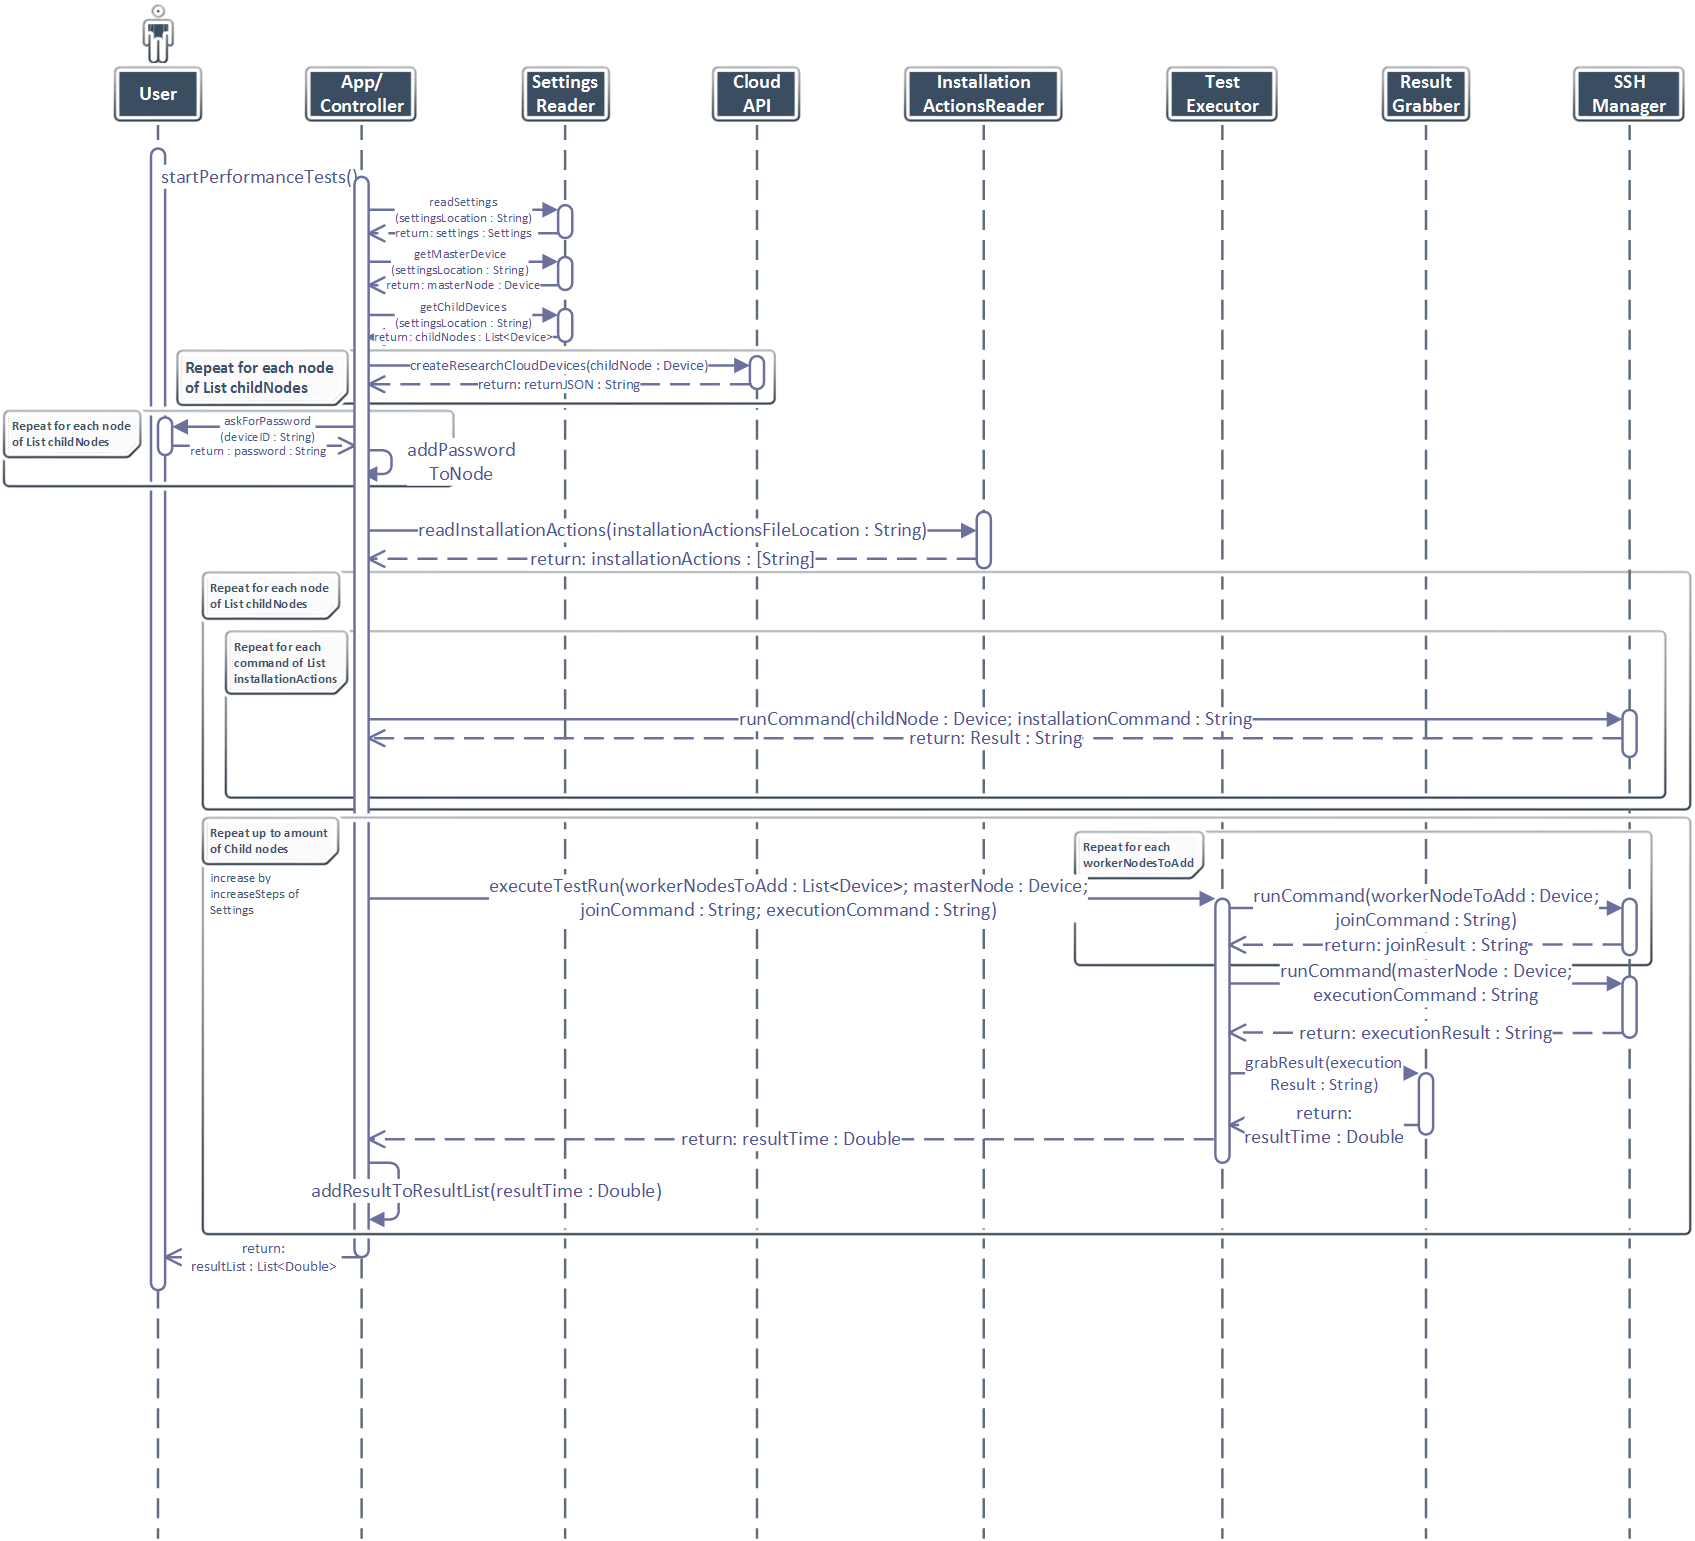
\includegraphics[width=\textheight/20*15]{images/testing_software_sequence_diagram.png}
}
\end{figure}

	
\end{document}
